% Provenance (never printed): cycle 3 / 6e "La planete Terre" (rocks and
% minerals; the three rock families; recognising common rocks); see
% sources/book1/PROVENANCE.md. Book 1, grade 6, chapter 3.
% Vocabulary guard: "magma" not before g7.2 (here "molten rock");
% "sediment" not before g7.4 (here "grains of sand and mud").
\chapter{चट्टानें और खनिज}\label{ch:g6:rocks-and-minerals}

सैम एक हाथ-लेंस लेकर रसोई के काउंटर पर झुकता है। चमकाया हुआ पत्थर, जो दूर से धूसर
दिखता है, कणों की एक भीड़ बन जाता है: गुलाबी कण, सफ़ेद कण, काँच जैसे धूसर कण और
नन्हे काले कण जो रोशनी पड़ने पर चमकते हैं। हर कण के समतल, चमकीले फलक हैं, और कण
किसी पहेली के टुकड़ों की तरह आपस में फ़िट बैठते हैं। ये क्या
हैं?

\begin{omfigure}
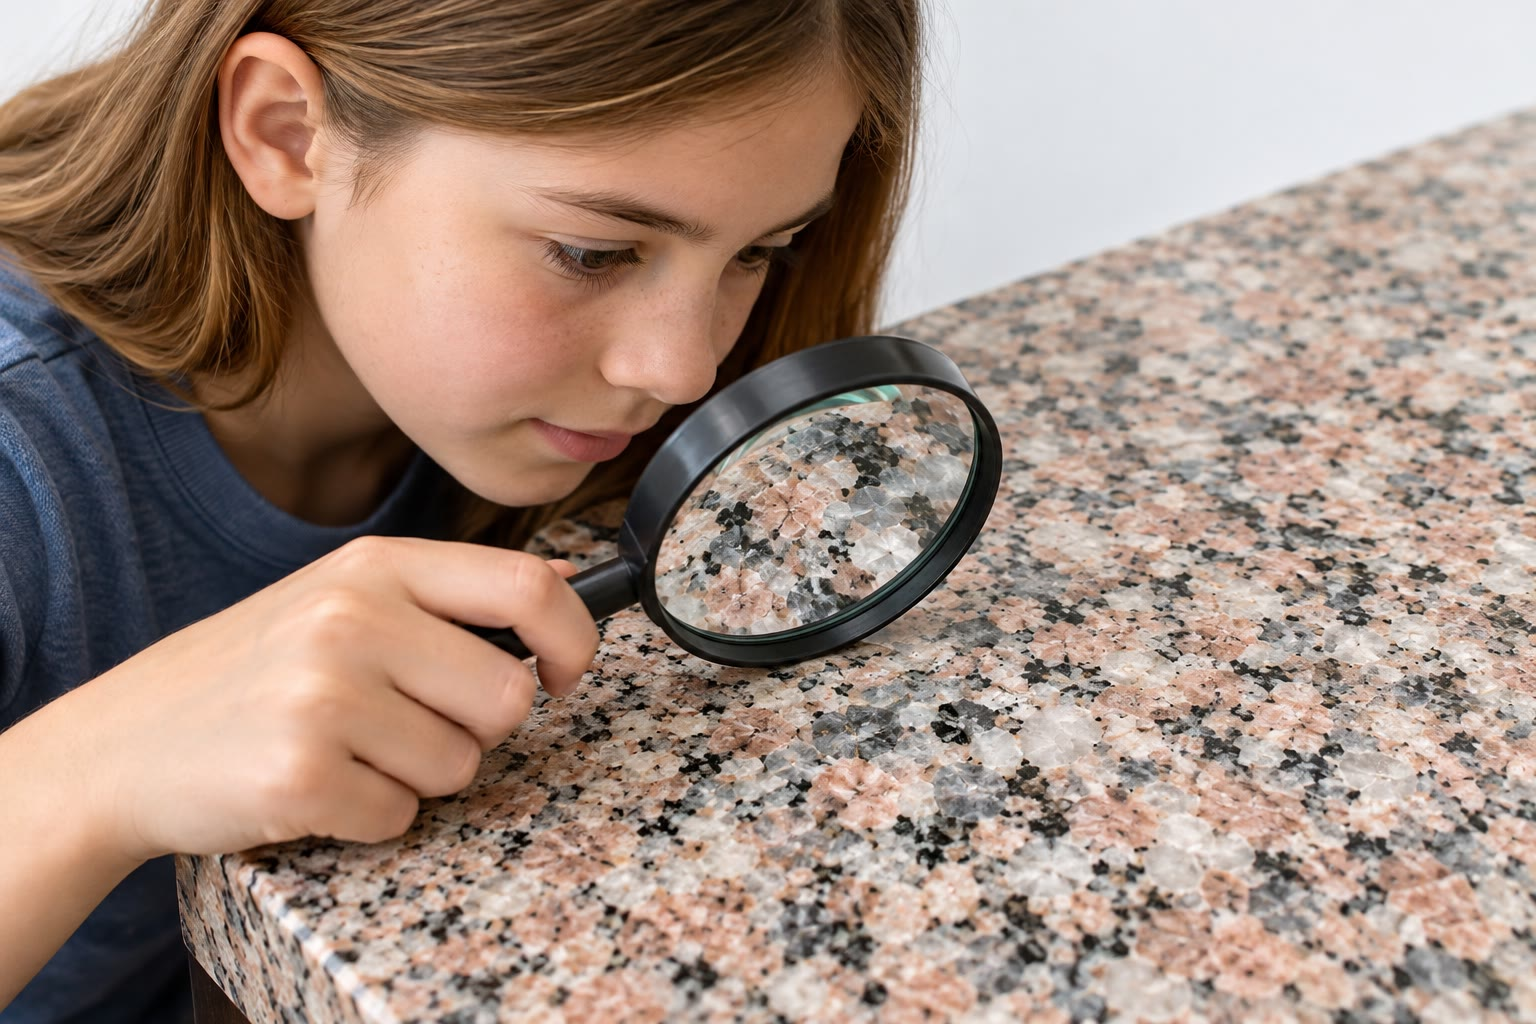
\includegraphics[width=0.6\linewidth]{images/book1/ai/g6-hand-lens-worktop.jpg}

{\small हाथ-लेंस से धब्बेदार पत्थर के एक काउंटर को देखना। (AI
चित्रण।)}
\end{omfigure}

\begin{recall}
\omterm{def:g3:stones-pebbles-sand:rock}{चट्टानें} पृथ्वी की भूपर्पटी का कठोर पदार्थ हैं: उन्हें तोड़कर पत्थर बनाए जा सकते
हैं, \omterm{def:g1:landscapes-around-us:water}{नदियाँ} उन्हें लुढ़काकर \omterm{def:g3:stones-pebbles-sand:pebble}{कंकड़} बना देती हैं, और पीसकर \omterm{def:g3:stones-pebbles-sand:sand}{रेत}
(\cref{ch:g3:stones-pebbles-sand})। पानी, बर्फ़ और हवा \omterm{def:g3:stones-pebbles-sand:rock}{चट्टानों} को घिसते हैं
(\omterm{def:g5:water-shapes-the-land:weathering}{अपक्षय}), टुकड़ों को दूर ले जाते हैं (\omterm{def:g5:water-shapes-the-land:erosion}{अपरदन}) और उन्हें और नीचे गिरा देते हैं
(\omterm{def:g5:water-shapes-the-land:deposition}{निक्षेपण}) (\cref{ch:g5:water-shapes-the-land})। \omterm{def:g4:volcanoes-earthquakes-first-look:volcano}{ज्वालामुखी} पर पिघली
\omterm{def:g3:stones-pebbles-sand:rock}{चट्टान} \omterm{def:g4:volcanoes-earthquakes-first-look:eruption}{लावा} बनकर निकलती है (\cref{ch:g4:volcanoes-earthquakes-first-look})।
\end{recall}

\section{चट्टान खनिजों से बनी होती है}

काउंटर के कण \omterm{def:g6:rocks-and-minerals:mineral}{खनिज} हैं, और पत्थर एक ग्रेनाइट है।

\begin{definition}[खनिज]\label{def:g6:rocks-and-minerals:mineral}
\emph{खनिज}\index{खनिज} एक प्राकृतिक ठोस पदार्थ है, जिसे जीवों ने नहीं बनाया, जिसकी
बनावट हमेशा एक-सी होती है और जिसके परमाणु एक नियमित ढंग से सजे होते हैं।
\emph{\omterm{def:g3:stones-pebbles-sand:rock}{चट्टान}} एक खनिज से या, ज़्यादातर, आपस में चिपके कई
खनिजों से बनी होती है।
% ledger: usgs:mineral-rock
\end{definition}

ग्रेनाइट ज़्यादातर तीन \omterm{def:g6:rocks-and-minerals:mineral}{खनिजों} से बना है: \emph{फ़ेल्डस्पार} (गुलाबी या सफ़ेद),
\emph{क्वार्ट्ज़} (धूसर और काँच जैसा) और \emph{अभ्रक} (काला या चाँदी जैसा, पतली
चमकीली परतों में)। दूसरी \omterm{def:g3:stones-pebbles-sand:rock}{चट्टानें} एक ही \omterm{def:g6:rocks-and-minerals:mineral}{खनिज} से बनी होती हैं: उदाहरण के लिए,
चूना पत्थर लगभग केवल कैल्साइट से बना है।
% ledger: nps:granite-minerals, usgs:mineral-rock

\begin{omfigure}
\begin{minipage}[c]{0.5\linewidth}\centering
\begin{tikzpicture}
  \begin{axis}[axis equal image, hide axis, width=\linewidth,
      xmin=0, xmax=6, ymin=0, ymax=4]
    \addplot[fill=orange!35!pink, draw=black!55, line width=0.4pt]
      table {figdata/out/grade-6-granite_mosaic-feldspar.dat};
    \addplot[fill=black!12, draw=black!55, line width=0.4pt]
      table {figdata/out/grade-6-granite_mosaic-quartz.dat};
    \addplot[fill=black!85, draw=black!55, line width=0.4pt]
      table {figdata/out/grade-6-granite_mosaic-mica.dat};
  \end{axis}
\end{tikzpicture}

{\small \tikz\fill[orange!35!pink, draw=black!55] (0,0) rectangle (0.25,0.18); फ़ेल्डस्पार\quad
\tikz\fill[black!12, draw=black!55] (0,0) rectangle (0.25,0.18); क्वार्ट्ज़\quad
\tikz\fill[black!85] (0,0) rectangle (0.25,0.18); अभ्रक}
\end{minipage}\hfill
\begin{minipage}[c]{0.46\linewidth}\centering
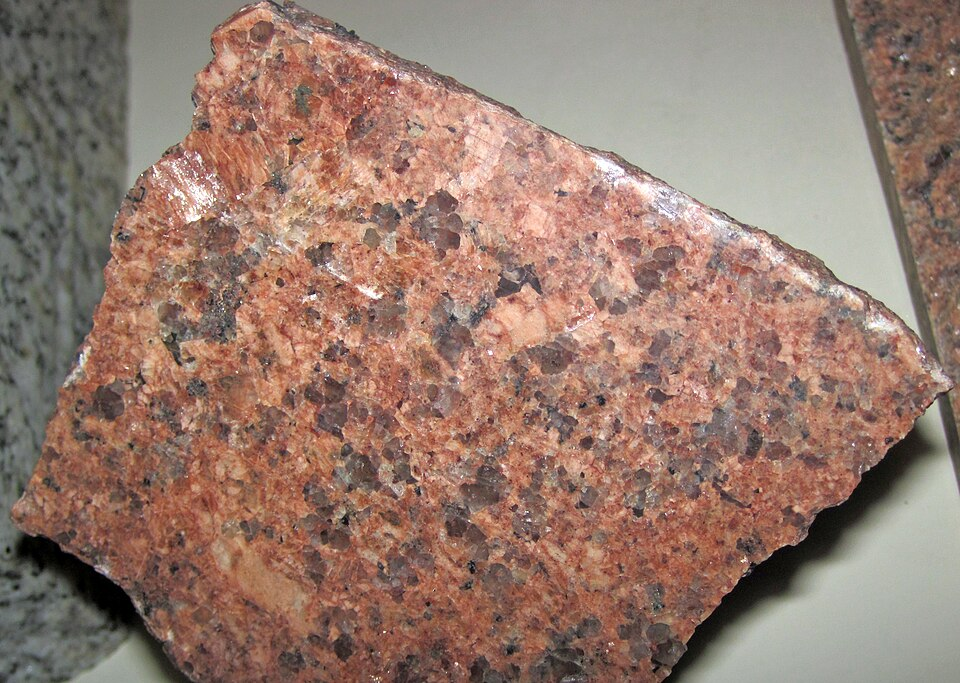
\includegraphics[width=\linewidth]{images/book1/g6-granite.jpg}
\end{minipage}

\smallskip
{\small बाएँ: कणों की पच्चीकारी के रूप में बना ग्रेनाइट, हर कण एक \omterm{def:g6:rocks-and-minerals:mineral}{खनिज}
(बड़ा करके, पैमाने पर नहीं)। दाएँ: एक असली गुलाबी ग्रेनाइट, लगभग एक हथेली
के आकार का। (फ़ोटो: जेम्स सेंट~जॉन, CC BY 2.0, विकिमीडिया कॉमन्स के ज़रिए।)}
% ledger: nps:granite-minerals, commons:jsj-rocks (figdata/grade-6/granite_mosaic.py)
\end{omfigure}

\section{क्रिस्टल}

लेंस के नीचे बहुत-से \omterm{def:g6:rocks-and-minerals:mineral}{खनिज} कणों में समतल, चमकीले फलक और सीधे किनारे दिखते हैं। जहाँ
किसी \omterm{def:g6:rocks-and-minerals:mineral}{खनिज} को \omterm{def:g3:stones-pebbles-sand:rock}{चट्टान} के किसी खोखले में खुलकर बढ़ने की जगह मिली है, वहाँ वह एक क्रिस्टल
बनाता है: समतल फलकों से घिरा, नियमित आकार का एक ठोस। उसका आकार उसके परमाणुओं की
नियमित सजावट से आता है, जिसका अध्ययन रसायन की पुस्तकों में होता है। उदाहरण के लिए,
क्वार्ट्ज़ का क्रिस्टल छह भुजाओं वाला एक स्तंभ है जो एक नोक में ख़त्म होता है; अभ्रक का
क्रिस्टल काग़ज़ से भी पतली
परतों में अलग हो जाता है।

\begin{omfigure}
\begin{minipage}[c]{0.2\linewidth}\centering
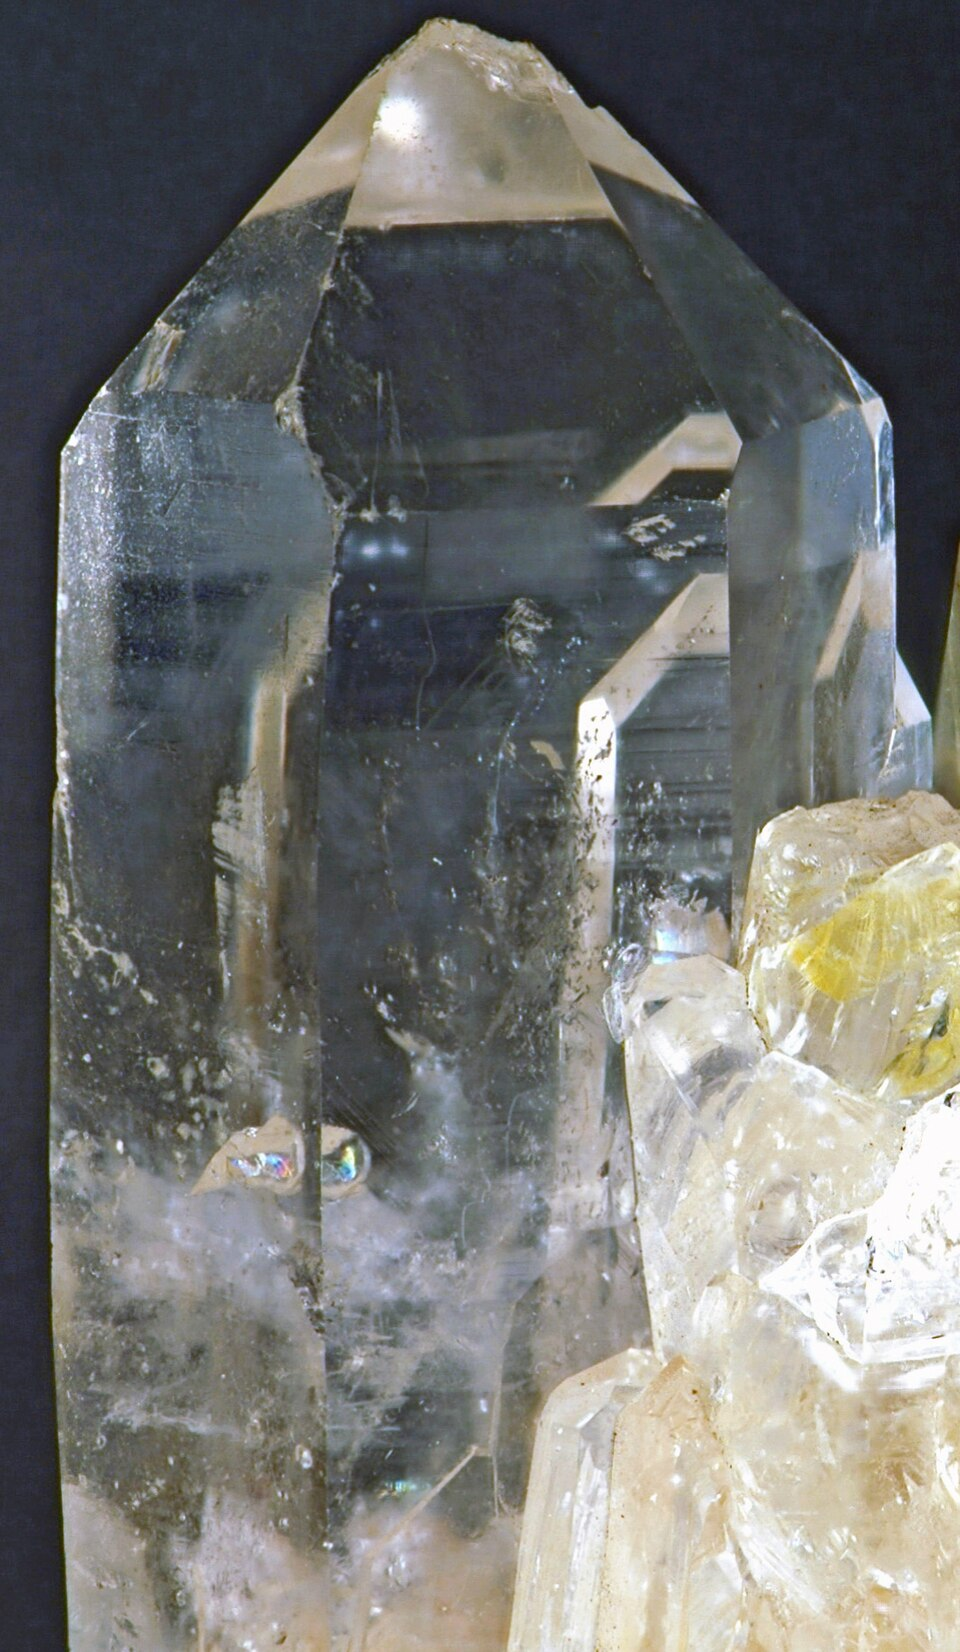
\includegraphics[height=4.2cm]{images/book1/g6-quartz.jpg}
\end{minipage}\hfill
\begin{minipage}[c]{0.44\linewidth}\centering
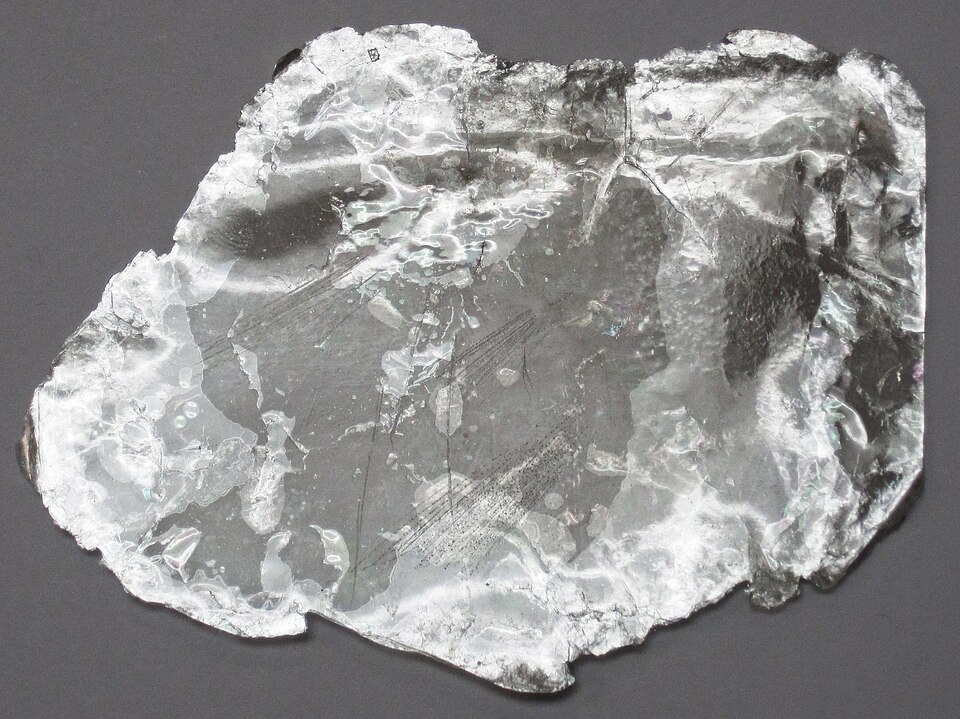
\includegraphics[height=4.2cm]{images/book1/g6-mica.jpg}
\end{minipage}\hfill
\begin{minipage}[c]{0.28\linewidth}
{\small बाएँ: क्वार्ट्ज़ का एक क्रिस्टल, अपने समतल फलकों के साथ। दाएँ: अभ्रक की
एक परत, एक ऐसा \omterm{def:g6:rocks-and-minerals:mineral}{खनिज} जो बहुत पतली परतों में अलग हो जाता है। (फ़ोटो: जेम्स
सेंट~जॉन, CC BY 2.0, विकिमीडिया कॉमन्स के ज़रिए।)}
% ledger: commons:jsj-rocks
\end{minipage}
\end{omfigure}

ग्रेनाइट में कण एक-दूसरे से दबे-दबे बढ़े, इसलिए उनके आकार सुघड़ नहीं हैं: वे एक पहेली
की तरह आपस में फ़िट बैठते हैं। उनका आकार एक कहानी कहता है। ग्रेनाइट ज़मीन के बहुत
नीचे बनता है, जहाँ पिघली \omterm{def:g3:stones-pebbles-sand:rock}{चट्टान} बहुत धीरे ठंडी होती है: उसके कणों को इतना बड़ा होने
का समय मिलता है कि वे आँख से दिख सकें। जो पिघली \omterm{def:g3:stones-pebbles-sand:rock}{चट्टान} सतह पर, \omterm{def:g4:volcanoes-earthquakes-first-look:eruption}{लावा} के रूप में,
जल्दी ठंडी होती है, उससे ऐसी \omterm{def:g3:stones-pebbles-sand:rock}{चट्टानें} बनती हैं जिनके कण देखने के लिए
बहुत छोटे होते हैं।
% ledger: usgs:mineral-rock

\section{चट्टानों के तीन परिवार}

भूवैज्ञानिक \omterm{def:g3:stones-pebbles-sand:rock}{चट्टानों} को तीन परिवारों में बाँटते हैं, उनके रंग से नहीं, बल्कि इस
आधार पर कि वे कैसे बनीं।

\begin{definition}[चट्टानों के तीन परिवार]\label{def:g6:rocks-and-minerals:rock-families}
\emph{आग्नेय चट्टान}\index{आग्नेय चट्टान} तब बनती है जब पिघली \omterm{def:g3:stones-pebbles-sand:rock}{चट्टान} ठंडी होकर
ठोस बन जाती है: ज़मीन के बहुत नीचे ग्रेनाइट, \omterm{def:g4:volcanoes-earthquakes-first-look:eruption}{लावा} से बेसाल्ट।
\emph{अवसादी चट्टान}\index{अवसादी चट्टान} पृथ्वी की सतह पर \omterm{def:g3:stones-pebbles-sand:sand}{रेत} और \omterm{def:g3:stones-pebbles-sand:sand}{कीचड़} के
कणों से, या जीवों के खोलों से, बनती है, जो परतों में बिछकर फिर कठोर हो जाते हैं:
बलुआ पत्थर, शेल, चूना पत्थर।
\emph{कायांतरित चट्टान}\index{कायांतरित चट्टान} वह \omterm{def:g3:stones-pebbles-sand:rock}{चट्टान} है जो ज़मीन के बहुत
नीचे ताप और दाब से, बिना पिघले, बदल गई है: संगमरमर
(चूना पत्थर से), स्लेट (शेल से)।
% ledger: usgs:mineral-rock, usgs:sedimentary, usgs:metamorphic, geo:marble, geo:slate
\end{definition}

\emph{आग्नेय} नाम संस्कृत के शब्द ``अग्नि'' से आया है, जिसका अर्थ है आग। \omterm{def:g6:rocks-and-minerals:rock-families}{अवसादी
चट्टानों} में अक्सर परतें दिखती हैं, एक के ऊपर एक, किसी पुस्तक के पन्नों की तरह।
\omterm{def:g6:rocks-and-minerals:rock-families}{कायांतरित चट्टानें} अक्सर दबी और मुड़ी हुई होती हैं; कुछ, जैसे स्लेट, समतल
परतों में अलग हो जाती हैं।
% ledger: usgs:mineral-rock, usgs:sedimentary, usgs:metamorphic

बहुत-सी \omterm{def:g6:rocks-and-minerals:rock-families}{अवसादी चट्टानें} उन कणों से बनी हैं जिन्हें तुमने
\cref{ch:g3:stones-pebbles-sand} में आकार के हिसाब से छाँटा था: \omterm{def:g3:stones-pebbles-sand:pebble}{कंकड़} और \omterm{def:g3:stones-pebbles-sand:pebble}{बजरी}, \omterm{def:g3:stones-pebbles-sand:sand}{रेत},
\omterm{def:g3:stones-pebbles-sand:sand}{कीचड़}। एक बार दब जाने पर कण अपना पानी खो देते हैं और एक प्राकृतिक सीमेंट से आपस
में चिपक जाते हैं। कणों का आकार \omterm{def:g3:stones-pebbles-sand:rock}{चट्टान} को उसका नाम देता है।
% ledger: usgs:sedimentary, usgs:wentworth

\begin{omfigure}
\begin{tikzpicture}[
    col/.style={draw=black!60, rounded corners=2pt, minimum width=3.6cm, minimum height=1.9cm},
    lab/.style={font=\scriptsize, align=center}]
  % gravel -> conglomerate
  \node[col, fill=omLithCongl!50] (g) at (0,0) {};
  \foreach \x/\y/\r in {-1.2/0.4/0.32, -0.4/-0.3/0.4, 0.5/0.35/0.3, 1.25/-0.35/0.33, 0.2/-0.55/0.18, -1.3/-0.5/0.22}
    \fill[gray!55, draw=black!60] (\x,\y) circle (\r);
  \node[lab, above=2pt] at (g.north) {\textbf{बजरी}\\ 2~mm से ज़्यादा};
  \node[lab, below=3pt] (cg) at (g.south) {$\downarrow$ दबी और जुड़ी\\ \textbf{कांग्लोमरेट}};
    % sand -> sandstone
  \pgfmathsetseed{7}

  \node[col, fill=omLithSand!60] (s) at (4.2,0) {};
  \foreach \i in {1,...,70} \fill[brown!60!black] ({4.2+1.65*rand},{0.82*rand}) circle (0.045);
  \node[lab, above=2pt] at (s.north) {\textbf{रेत}\\ 2~mm से $\frac{1}{16}$~mm तक};
  \node[lab, below=3pt] at (s.south) {$\downarrow$ दबी और जुड़ी\\ \textbf{बलुआ पत्थर}};
  % mud -> shale
  \node[col, fill=omLithShale!70] (m) at (8.4,0) {};
  \foreach \y in {-0.75,-0.5,...,0.8} \draw[black!35, line width=0.3pt] (6.75,\y) -- (10.05,\y);
  \node[lab, above=2pt] at (m.north) {\textbf{कीचड़} (गाद और चिकनी मिट्टी)\\ $\frac{1}{16}$~mm से कम};
  \node[lab, below=3pt] at (m.south) {$\downarrow$ दबा और दाबा गया\\ \textbf{शेल}};
\end{tikzpicture}

{\small अपने कणों के आकार के नाम पर तीन \omterm{def:g6:rocks-and-minerals:rock-families}{अवसादी चट्टानें} (कण बहुत बड़े करके
दिखाए गए; \omterm{def:g3:stones-pebbles-sand:sand}{रेत} डिब्बे के पैमाने पर, \omterm{def:g3:stones-pebbles-sand:pebble}{बजरी} उससे बड़ी)।}
% ledger: usgs:wentworth, usgs:sedimentary
\end{omfigure}

\begin{inthefield}[किसी शहर के पत्थर पढ़ना]
शहर खुले आसमान के नीचे \omterm{def:g3:stones-pebbles-sand:rock}{चट्टानों} के संग्रह हैं। किसी बड़े के साथ पुरानी दीवारों,
सीढ़ियों, मूर्तियों, गिरजाघरों के अग्रभागों और फ़र्शों के पास से गुज़रो, और ध्यान से देखो,
बिना कुछ खरोंचे या तोड़े। कुछ फ़ुटपाथ-किनारे और सीढ़ियाँ ग्रेनाइट की हैं: उसका काँच जैसा क्वार्ट्ज़ और चमकीला अभ्रक खोजो। बहुत-सी पुरानी दीवारें और अग्रभाग चूना पत्थर या बलुआ पत्थर के हैं: खोल खोजो, या बलुआ पत्थर के किसी गिरे हुए
भुरभुरे टुकड़े पर उँगली की नोक रगड़कर \omterm{def:g3:stones-pebbles-sand:sand}{रेत} महसूस करो। छतें स्लेट की हो सकती हैं, पतली परतों में बँटी।
एक कॉपी में लिखो कि हर पत्थर कहाँ है, उसका रंग, उसके कण, और वह परिवार जिसका
तुम्हें लगता है कि वह है; एक फ़ोटो बाद में इस अध्याय की तालिका से तुलना करने में
मदद करता है।
\end{inthefield}

\section{शैल चक्र}

\omterm{def:g3:stones-pebbles-sand:rock}{चट्टानें} शाश्वत नहीं हैं। ग्रेनाइट का एक \omterm{def:g1:landscapes-around-us:landform}{पर्वत} धीरे-धीरे अपक्षयित होता है; उसके कण
\omterm{def:g1:landscapes-around-us:water}{नदियाँ} \omterm{def:g2:water-on-earth:ocean}{समुद्र} तक ले जाती हैं और वहाँ परतों में बिछा देती हैं; और गहरे और गहरे
दबकर परतें कठोर होकर बलुआ पत्थर बन जाती हैं। अगर बलुआ पत्थर और भी गहरे ले जाया
जाए, तो ताप और दाब उसे एक \omterm{def:g6:rocks-and-minerals:rock-families}{कायांतरित चट्टान} में बदल देते हैं; और गहरे, वह पिघल सकता
है, और पिघली \omterm{def:g3:stones-pebbles-sand:rock}{चट्टान}, ठंडी होकर, एक नई \omterm{def:g6:rocks-and-minerals:rock-families}{आग्नेय चट्टान} बनाती है। थोड़ा-थोड़ा करके,
लाखों वर्षों में, \omterm{def:g3:stones-pebbles-sand:rock}{चट्टानों} का पदार्थ
घूमता रहता है।
% ledger: usgs:sedimentary, usgs:metamorphic

\begin{definition}[शैल चक्र]\label{def:g6:rocks-and-minerals:rock-cycle}
\emph{शैल चक्र}\index{शैल चक्र} वह अंतहीन यात्रा है जिससे हर परिवार की
\omterm{def:g3:stones-pebbles-sand:rock}{चट्टानें} धीरे-धीरे दूसरे परिवारों की \omterm{def:g3:stones-pebbles-sand:rock}{चट्टानों} में बदलती हैं:
सतह पर \omterm{def:g5:water-shapes-the-land:weathering}{अपक्षय} और \omterm{def:g5:water-shapes-the-land:erosion}{अपरदन} से, दबने और कठोर होने से, ताप
और दाब से, पिघलने और ठंडा होने से।
\end{definition}

\begin{omfigure}
\begin{tikzpicture}[
    fam/.style={draw, rounded corners=4pt, thick, align=center, minimum width=3.2cm,
                minimum height=1.0cm, font=\small\bfseries},
    stage/.style={draw, dashed, rounded corners=4pt, align=center, minimum width=3.0cm,
                  minimum height=0.9cm, font=\small},
    arr/.style={-{Stealth[length=2.6mm]}, thick},
    lab/.style={font=\scriptsize, align=center, fill=white, inner sep=1.5pt}]
  \node[fam, fill=omLithGranite!60] (ign) at (0,3.6) {आग्नेय चट्टानें\\[-1pt]{\normalfont\scriptsize ग्रेनाइट, बेसाल्ट}};
  \node[stage, fill=orange!15] (grains) at (6.6,3.6) {रेत और कीचड़\\के कण};
  \node[fam, fill=omLithSand!70] (sed) at (6.6,0) {अवसादी चट्टानें\\[-1pt]{\normalfont\scriptsize बलुआ पत्थर, शेल, चूना पत्थर}};
  \node[fam, fill=omLithSchist!60] (met) at (0,0) {कायांतरित चट्टानें\\[-1pt]{\normalfont\scriptsize संगमरमर, स्लेट}};
  \node[stage, fill=red!12] (melt) at (-4.2,1.8) {गहराई में\\पिघली चट्टान};
  \draw[arr] (ign) -- node[lab, above] {अपक्षय\\और अपरदन} (grains);
  \draw[arr] (grains) -- node[lab, right] {परतों में बिछे,\\दबे, कठोर हुए} (sed);
  \draw[arr] (sed) -- node[lab, below=2pt] {ताप और दाब,\\गहराई में} (met);
  \draw[arr] (met) -- node[lab, below left] {पिघलना} (melt);
  \draw[arr] (melt) -- node[lab, above left] {ठंडा होना} (ign);
  \draw[arr, black!55] (met.north east) to[bend left=12] node[lab, pos=0.45, left=4pt, text=black!60] {अपक्षय} ([xshift=-6pt]grains.south west);
  \draw[arr, black!55] (sed.north west) to[bend left=10] (grains.south west);
\end{tikzpicture}

{\small \omterm{def:g6:rocks-and-minerals:rock-cycle}{शैल चक्र}। हर तीर में हज़ारों से लाखों वर्ष लगते हैं। सतह पर आने वाली कोई भी
\omterm{def:g3:stones-pebbles-sand:rock}{चट्टान} अपक्षयित हो सकती है (धूसर
तीर)।}
% ledger: usgs:sedimentary, usgs:metamorphic, usgs:mineral-rock
\end{omfigure}

\section{आम चट्टानों को पहचानना}

यहाँ सात \omterm{def:g3:stones-pebbles-sand:rock}{चट्टानें} हैं जो अक्सर इमारतों, फ़ुटपाथों और \omterm{def:g1:landscapes-around-us:landscape}{भूदृश्यों} में
मिलती हैं।

\begin{omfigure}
\newcommand{\gsixrock}[2]{\begin{minipage}[t]{0.235\linewidth}\centering
  \includegraphics[width=\linewidth, height=0.72\linewidth, keepaspectratio=false]{images/book1/#1}\\[1pt]
  {\footnotesize #2}\end{minipage}}
\gsixrock{g6-granite.jpg}{ग्रेनाइट}\hfill
\gsixrock{g6-basalt.jpg}{बेसाल्ट}\hfill
\gsixrock{g6-sandstone.jpg}{बलुआ पत्थर}\hfill
\gsixrock{g6-limestone.jpg}{चूना पत्थर (खोलों के साथ)}\par\medskip
\gsixrock{g6-shale.jpg}{शेल}\hspace{0.02\linewidth}%
\gsixrock{g6-marble.jpg}{संगमरमर}\hspace{0.02\linewidth}%
\gsixrock{g6-slate-roof.jpg}{स्लेट, एक छत पर}

\medskip
{\small सात आम \omterm{def:g3:stones-pebbles-sand:rock}{चट्टानें}। (फ़ोटो: जेम्स सेंट~जॉन, CC BY 2.0; छत:
ओयविंद होल्मस्टाड, CC0; विकिमीडिया कॉमन्स के ज़रिए।)}
% ledger: commons:jsj-rocks, commons:roof-slates
\end{omfigure}

\begin{center}
\small
\begin{tabular}{>{\raggedright\arraybackslash}p{0.13\linewidth}>{\raggedright\arraybackslash}p{0.15\linewidth}>{\raggedright\arraybackslash}p{0.6\linewidth}}
\hline
\omterm{def:g3:stones-pebbles-sand:rock}{चट्टान} & परिवार & क्या खोजें\\
\hline
ग्रेनाइट & आग्नेय & कई रंगों के बड़े कण: गुलाबी या सफ़ेद फ़ेल्डस्पार, धूसर काँच जैसा क्वार्ट्ज़, काला चमकीला अभ्रक\\
बेसाल्ट & आग्नेय & गहरे धूसर से काला, कण देखने के लिए बहुत छोटे, अक्सर गैस के बुलबुलों से बने छोटे गोल छेद\\
बलुआ पत्थर & अवसादी & \omterm{def:g3:stones-pebbles-sand:sand}{रेत} के कण जिन्हें तुम महसूस कर सकते हो, रेगमाल की तरह खुरदरा\\
चूना पत्थर & अवसादी & हल्के रंग का, अक्सर खोलों के साथ; तनु अम्ल की एक बूँद से बुदबुदाता है\\
शेल & अवसादी & बहुत महीन और नरम, कठोर हुए \omterm{def:g3:stones-pebbles-sand:sand}{कीचड़} (चिकनी मिट्टी) से बना; पतली परतों में\\
संगमरमर & कायांतरित & सफ़ेद या रंगीन, चमकीले क्रिस्टलों से बना जो चीनी की तरह झिलमिलाते हैं; अम्ल से बुदबुदाता है\\
स्लेट & कायांतरित & धूसर, बहुत महीन, पतली, कठोर, समतल परतों में अलग होता है\\
\hline
\end{tabular}
% ledger: nps:granite-minerals, geo:basalt, usgs:sedimentary, geo:limestone, geo:marble, geo:slate
\end{center}

\begin{safety}
अम्ल की जाँच केवल कोई बड़ा, चश्मा और दस्ताने पहनकर, बहुत तनु अम्ल से करता है। किसी
\omterm{def:g3:stones-pebbles-sand:rock}{चट्टान} या चूर्ण को कभी मत चखो, और किसी औज़ार से \omterm{def:g3:stones-pebbles-sand:rock}{चट्टानें} कभी मत तोड़ो: हाथ-लेंस से
देखना बहुत कुछ बता देता है।
% ledger: geo:limestone
\end{safety}

कुंजी प्रश्नों की एक सूची है, हर प्रश्न के दो जवाबों के साथ, जो क़दम-दर-क़दम किसी
\omterm{def:g3:stones-pebbles-sand:rock}{चट्टान} के नाम तक ले जाती है।

\begin{omfigure}
\begin{tikzpicture}[
    q/.style={draw, rounded corners=3pt, fill=omRecall!10, align=center, text width=3.7cm,
              font=\scriptsize, inner sep=3pt},
    r/.style={draw, rounded corners=3pt, thick, fill=omLithSand!40, font=\scriptsize\bfseries,
              align=center, minimum width=1.7cm, inner sep=3pt},
    arr/.style={-{Stealth[length=2mm]}, thick}, yn/.style={font=\scriptsize\itshape, fill=white, inner sep=1pt}]
  \node[q] (q1) at (0,0) {क्या वह तनु अम्ल की एक बूँद से बुदबुदाती है?};
  \node[q] (q2) at (-3.4,-1.6) {क्या तुम्हें खोल दिखते हैं, या वह फीकी और महीन दिखती है?};
  \node[r] (lime) at (-4.8,-3.4) {चूना पत्थर};
  \node[r, align=center] (marb) at (-2.0,-3.4) {संगमरमर\\[-1pt]{\normalfont\tiny चमकीले क्रिस्टल}};
  \node[q] (q3) at (3.2,-1.6) {क्या तुम्हें कई रंगों के कण दिखते हैं, गुलाबी, धूसर, काले?};
  \node[r] (gran) at (6.9,-1.6) {ग्रेनाइट};
  \node[q] (q4) at (3.2,-3.2) {गहरी, कण देखने के लिए बहुत छोटे, छोटे गोल छेद?};
  \node[r] (bas) at (6.9,-3.2) {बेसाल्ट};
  \node[q] (q5) at (3.2,-4.8) {रेगमाल की तरह खुरदरी, रेत के कणों से बनी?};
  \node[r] (sand) at (6.9,-4.8) {बलुआ पत्थर};
  \node[q] (q6) at (3.2,-6.4) {कठोर, पतली समतल परतों में अलग होती?};
  \node[r] (slat) at (6.9,-6.4) {स्लेट};
  \node[r] (shal) at (3.2,-7.8) {शेल};
  \draw[arr] (q1) -| node[yn, pos=0.25] {हाँ} (q2);
  \draw[arr] (q1) -| node[yn, pos=0.25] {नहीं} (q3);
  \draw[arr] (q2.south-|lime) -- node[yn, right] {हाँ} (lime);
  \draw[arr] (q2.south-|marb) -- node[yn, right] {नहीं} (marb);
  \foreach \a/\b in {q3/gran, q4/bas, q5/sand, q6/slat}{\draw[arr] (\a) -- node[yn, above] {हाँ} (\b);}
  \foreach \a/\b in {q3/q4, q4/q5, q5/q6, q6/shal}{\draw[arr] (\a) -- node[yn, right] {नहीं} (\b);}
\end{tikzpicture}

{\small तालिका की सात \omterm{def:g3:stones-pebbles-sand:rock}{चट्टानों} के लिए एक कुंजी। ऊपर से शुरू करो और हर प्रश्न का
जवाब हाँ या नहीं में दो।}
% ledger: geo:limestone, geo:marble, nps:granite-minerals, geo:basalt, usgs:sedimentary, geo:slate
\end{omfigure}

\paragraph{कठोरता।} एक और सुराग किसी \omterm{def:g6:rocks-and-minerals:mineral}{खनिज} को पहचानने में मदद करता है: उसे कितनी
आसानी से खरोंचा जा सकता है।

\begin{definition}[कठोरता और मोह्स पैमाना]\label{def:g6:rocks-and-minerals:hardness}
किसी \omterm{def:g6:rocks-and-minerals:mineral}{खनिज} की \emph{कठोरता}\index{कठोरता} यह है कि वह खरोंचे जाने का कितना अच्छा
विरोध करता है: एक \omterm{def:g6:rocks-and-minerals:mineral}{खनिज} अपने से हर नरम \omterm{def:g6:rocks-and-minerals:mineral}{खनिज} को खरोंचता है और अपने से हर कठोर \omterm{def:g6:rocks-and-minerals:mineral}{खनिज}
से खरोंचा जाता है। \emph{मोह्स पैमाना}\index{मोह्स पैमाना} दस संदर्भ \omterm{def:g6:rocks-and-minerals:mineral}{खनिजों} के साथ
कठोरता को 1 से 10 तक क्रम देता है, टैल्क (1) से, जो सबसे नरम है,
हीरे (10) तक, जो सबसे कठोर है।
% ledger: nps:mohs-ladder, nps:mohs-testers
\end{definition}

\begin{omfigure}
\begin{tikzpicture}[x=1cm, y=0.62cm]
  \draw[thick, black!60] (0,0.5) -- (0,10.5);
  \foreach \n/\m in {1/टैल्क, 2/जिप्सम, 3/कैल्साइट, 4/फ़्लोराइट, 5/एपेटाइट,
                     6/फ़ेल्डस्पार (ऑर्थोक्लेज़), 7/क्वार्ट्ज़, 8/पुखराज, 9/कोरंडम, 10/हीरा}{
    \fill[omRecall!25, draw=black!50] (-0.32,\n-0.32) rectangle (0.32,\n+0.32);
    \node[font=\scriptsize\bfseries] at (0,\n) {\n};
    \node[font=\scriptsize, anchor=east] at (-0.5,\n) {\m};}
  \foreach \v/\t in {2.5/नाख़ून, 3.5/ताँबे का सिक्का, 5.5/काँच, 6.5/स्टील की कील}{
    \draw[red!70!black, thick] (0.4,\v) -- (1.0,\v);
    \node[font=\scriptsize, red!70!black, anchor=west] at (1.05,\v) {\t\ (लगभग \v)};}
  \node[font=\scriptsize\itshape, anchor=south] at (0,10.6) {ज़्यादा कठोर};
  \node[font=\scriptsize\itshape, anchor=north] at (0,0.4) {ज़्यादा नरम};
  \node[font=\scriptsize, align=left, anchor=west, text width=6.2cm] at (4.3,5.5)
    {नाख़ून टैल्क और जिप्सम को खरोंचता है, पर कैल्साइट को नहीं। ताँबे का सिक्का
     कैल्साइट को खरोंचता है। क्वार्ट्ज़ काँच और स्टील को खरोंचता है; चारों जाँचकों में से कोई भी क्वार्ट्ज़ को नहीं खरोंचता। अभ्रक, 2 से 3 पर, नाख़ून से
     बस खरोंचा जा सकता है।};
\end{tikzpicture}

{\small \omterm{def:g6:rocks-and-minerals:hardness}{मोह्स पैमाना} (बाएँ: दस संदर्भ \omterm{def:g6:rocks-and-minerals:mineral}{खनिज}) और चार
रोज़मर्रा के जाँचक (दाएँ, लाल में)।}
% ledger: nps:mohs-ladder, nps:mohs-testers, geo:mica-hardness
\end{omfigure}

\begin{method}[खरोंच जाँच]\label{met:g6:rocks-and-minerals:scratch}
\begin{enumerate}
  \item \omterm{def:g6:rocks-and-minerals:mineral}{खनिज} को अपने नाख़ून से खरोंचने की कोशिश करो, फिर ताँबे के एक
        सिक्के से। (काँच और स्टील का प्रयोग केवल कोई बड़ा करता है।)
  \item निशान को उँगली से रगड़ो: असली खरोंच बनी रहती है, जाँचक के चूर्ण का
        निशान मिट जाता है।
  \item \omterm{def:g6:rocks-and-minerals:hardness}{कठोरता} उस सबसे कठोर जाँचक की \omterm{def:g6:rocks-and-minerals:hardness}{कठोरता}, जो उसे नहीं खरोंचता, और उस सबसे
        नरम जाँचक की \omterm{def:g6:rocks-and-minerals:hardness}{कठोरता}, जो उसे खरोंचता है, के बीच होती है।
\end{enumerate}
\end{method}

\begin{example}[क्वार्ट्ज़ या कैल्साइट?]\label{ex:g6:rocks-and-minerals:quartz-calcite}
दो सफ़ेद \omterm{def:g6:rocks-and-minerals:mineral}{खनिज} एक-से दिखते हैं। पहला ताँबे के सिक्के से खरोंच जाता है:
उसकी \omterm{def:g6:rocks-and-minerals:hardness}{कठोरता} 3.5 से कम है; वह कैल्साइट (3) है। दूसरे पर स्टील की कील से खरोंच नहीं
पड़ती और वह काँच को खरोंचता है: उसकी \omterm{def:g6:rocks-and-minerals:hardness}{कठोरता}
6.5 से ज़्यादा है; संदर्भ \omterm{def:g6:rocks-and-minerals:mineral}{खनिजों} में वह क्वार्ट्ज़ (7) है।
% ledger: nps:mohs-ladder, nps:mohs-testers
\end{example}

\section{अभ्यास}

\begin{exercise}[$\star$]\label{exo:g6:rocks-and-minerals:1}
हर \omterm{def:g3:stones-pebbles-sand:rock}{चट्टान} किस परिवार की है: ग्रेनाइट, बलुआ पत्थर, संगमरमर, बेसाल्ट,
चूना पत्थर, स्लेट?
\end{exercise}

\begin{exercise}[$\star$]\label{exo:g6:rocks-and-minerals:2}
क्वार्ट्ज़ \omterm{def:g6:rocks-and-minerals:mineral}{खनिज} है या \omterm{def:g3:stones-pebbles-sand:rock}{चट्टान}? और ग्रेनाइट? अंतर को एक
वाक्य में समझाओ।
\end{exercise}

\begin{exercise}[$\star$]\label{exo:g6:rocks-and-minerals:3}
इन \omterm{def:g6:rocks-and-minerals:mineral}{खनिजों} को सबसे नरम से सबसे कठोर के क्रम में लगाओ: क्वार्ट्ज़,
टैल्क, हीरा, कैल्साइट। इनमें से कौन बाक़ी सबको खरोंच सकता है?
\end{exercise}

\begin{exercise}[$\star$]\label{exo:g6:rocks-and-minerals:4}
\emph{ठंडा होना}, \emph{ताप और दाब},
\emph{\omterm{def:g5:water-shapes-the-land:weathering}{अपक्षय}} शब्दों से उतारो और पूरा करो: ``पिघली \omterm{def:g3:stones-pebbles-sand:rock}{चट्टान} \ldots{} से \omterm{def:g6:rocks-and-minerals:rock-families}{आग्नेय चट्टान} बनती है।
चूना पत्थर \ldots{} से संगमरमर बनता है। ग्रेनाइट \ldots{} से \omterm{def:g3:stones-pebbles-sand:sand}{रेत} के कणों
में बदलता है।''
\end{exercise}

\begin{exercise}[$\star\star$]\label{exo:g6:rocks-and-minerals:5}
कुंजी का प्रयोग करो। (क) एक \omterm{def:g3:stones-pebbles-sand:rock}{चट्टान} अम्ल से नहीं बुदबुदाती; वह गहरी है, कण
देखने के लिए बहुत छोटे और छोटे गोल छेद। (ख) एक \omterm{def:g3:stones-pebbles-sand:rock}{चट्टान} अम्ल से बुदबुदाती है और
चीनी की तरह झिलमिलाते चमकीले क्रिस्टलों से बनी है। (ग) एक \omterm{def:g3:stones-pebbles-sand:rock}{चट्टान} नहीं
बुदबुदाती; वह रेगमाल की तरह खुरदरी है। हर \omterm{def:g3:stones-pebbles-sand:rock}{चट्टान} का नाम बताओ।
\end{exercise}

\begin{exercise}[$\star\star$]\label{exo:g6:rocks-and-minerals:6}
एक \omterm{def:g6:rocks-and-minerals:mineral}{खनिज} ताँबे के सिक्के से खरोंच जाता है पर नाख़ून से नहीं। उसकी \omterm{def:g6:rocks-and-minerals:hardness}{कठोरता} किन दो
मानों के बीच है? \omterm{def:g6:rocks-and-minerals:hardness}{मोह्स पैमाने} का कौन-सा संदर्भ \omterm{def:g6:rocks-and-minerals:mineral}{खनिज}
वह हो सकता है?
\end{exercise}

\begin{exercise}[$\star\star$]\label{exo:g6:rocks-and-minerals:7}
% exercise data: figdata/grade-6/granite_mosaic.py (33 / 21 / 6 grains)
इस अध्याय के ग्रेनाइट के चित्र में 60 कण हैं: 33
फ़ेल्डस्पार के, 21 क्वार्ट्ज़ के और 6 अभ्रक के। कणों का कितना प्रतिशत
क्वार्ट्ज़ है? फ़ेल्डस्पार? अभ्रक? जाँचो कि तीनों प्रतिशत जुड़कर
100~\% होते हैं।
\end{exercise}

\begin{exercise}[$\star\star$]\label{exo:g6:rocks-and-minerals:8}
ग्रेनाइट और बेसाल्ट दोनों \omterm{def:g6:rocks-and-minerals:rock-families}{आग्नेय चट्टानें} हैं। हम ग्रेनाइट के कणों को आँखों से क्यों
देख सकते हैं, पर बेसाल्ट के कणों को नहीं?
\end{exercise}

\begin{exercise}[$\star\star$]\label{exo:g6:rocks-and-minerals:9}
संगमरमर चूना पत्थर से बनता है। (क) हर एक किस परिवार का है?
(ख) चूना पत्थर के साथ क्या हुआ कि वह संगमरमर बन गया? (ग) दोनों अम्ल से
क्यों बुदबुदाते हैं?
\end{exercise}

\begin{exercise}[$\star\star$]\label{exo:g6:rocks-and-minerals:10}
\omterm{def:g6:rocks-and-minerals:hardness}{मोह्स पैमाने} की मदद से: (क) क्या क्वार्ट्ज़ काँच की एक बोतल को खरोंच सकता है? (ख) क्या
फ़्लोराइट? (ग) क्या स्टील की कील फ़ेल्डस्पार को खरोंच सकती है?
\end{exercise}

\begin{exercise}[$\star\star\star$]\label{exo:g6:rocks-and-minerals:11}
क्वार्ट्ज़ के एक कण की यात्रा, पाँच क़दमों में, ग्रेनाइट के एक \omterm{def:g1:landscapes-around-us:landform}{पर्वत} से एक \omterm{def:g6:rocks-and-minerals:rock-families}{कायांतरित
चट्टान} तक बताओ। हर क़दम पर प्रक्रिया का नाम बताओ, और शुरुआत और अंत की \omterm{def:g3:stones-pebbles-sand:rock}{चट्टान} का
परिवार।
\end{exercise}

\begin{exercise}[$\star\star\star$]\label{exo:g6:rocks-and-minerals:12}
एक धूसर काँच जैसा \omterm{def:g6:rocks-and-minerals:mineral}{खनिज} स्टील की कील से नहीं खरोंचा जाता, काँच को खरोंचता है,
और पुखराज से खरोंच जाता है। (क) \omterm{def:g6:rocks-and-minerals:hardness}{मोह्स पैमाने} पर उसकी \omterm{def:g6:rocks-and-minerals:hardness}{कठोरता} क्या है?
उसका नाम बताओ। (ख) \omterm{def:g3:stones-pebbles-sand:sand}{रेत} के कण लहरों और \omterm{def:g1:landscapes-around-us:water}{नदियों} से वर्षों तक लुढ़काए जाते हैं।
उसकी \omterm{def:g6:rocks-and-minerals:hardness}{कठोरता} की मदद से समझाओ कि इस \omterm{def:g6:rocks-and-minerals:mineral}{खनिज} के कण कैल्साइट या अभ्रक के
कणों से बहुत ज़्यादा समय तक क्यों टिकते हैं।
\end{exercise}

\section{समस्या: शहर के चौक के पत्थर}

\begin{problem}[{सप्ताहांत समस्या --- शहर के एक चौक की चट्टानें, उनमें सबसे
कठोर खनिज, और वहाँ चट्टानों के कितने परिवार हैं}]
\label{pb:g6:rocks-and-minerals:1}
% ledger: nps:granite-minerals, geo:limestone, geo:slate, geo:marble, nps:mohs-ladder, nps:mohs-testers, geo:mica-hardness
स्कूल की एक सैर पर कक्षा पुराने शहर के चौक के पत्थरों को देखती है
(केवल देखना: कोई स्मारकों को न तोड़ता है न खरोंचता है)। अध्यापक
\omterm{def:g6:rocks-and-minerals:hardness}{कठोरता} की जाँच के लिए संगतराश के आँगन से उन्हीं पत्थरों के ढीले टुकड़े
लाए हैं।

\smallskip
\noindent\textbf{फ़व्वारा}: उसके हौज़ में बड़े कण दिखते हैं, गुलाबी, सफ़ेद,
        धूसर और काँच जैसे, और काले और चमकीले।
\textbf{फ़र्श}: हल्के रंग की पटियाएँ जिनमें छोटे जीवाश्म
        खोल दिखते हैं; अध्यापक द्वारा एक ढीले टुकड़े पर डाली गई तनु अम्ल की एक बूँद
        बुदबुदाती है।
\textbf{नगर भवन की छत}: बहुत महीन कणों वाले एक पत्थर की पतली, समतल, धूसर
        परतें।
\textbf{मूर्ति}: चमकीले क्रिस्टलों से बना एक सफ़ेद पत्थर जो
        चीनी की तरह झिलमिलाता है; वह भी बुदबुदाता है।

\medskip
\noindent\textbf{भाग I --- फ़व्वारा, फ़र्श, छत।}
\begin{enumerate}
  \item फ़व्वारे की \omterm{def:g3:stones-pebbles-sand:rock}{चट्टान} और उसके परिवार का नाम बताओ। उसके तीनों
        \omterm{def:g6:rocks-and-minerals:mineral}{खनिजों} के नाम बताओ।
  \item फ़र्श की \omterm{def:g3:stones-pebbles-sand:rock}{चट्टान} और उसके परिवार का नाम बताओ। पत्थर में आने से पहले खोल
        क्या थे?
  \item छत की \omterm{def:g3:stones-pebbles-sand:rock}{चट्टान} और उसके परिवार का नाम बताओ। वह किस \omterm{def:g3:stones-pebbles-sand:rock}{चट्टान} से
        बनी?
  \item मूर्ति की \omterm{def:g3:stones-pebbles-sand:rock}{चट्टान} और उसके परिवार का नाम बताओ। वह किस \omterm{def:g3:stones-pebbles-sand:rock}{चट्टान} से
        बनी?
\end{enumerate}

\medskip
\noindent\textbf{भाग II --- कठोरता की एक जाँच।}
\begin{enumerate}[resume]
  \item अध्यापक फ़व्वारे के एक धूसर काँच जैसे कण को स्टील की कील से खरोंचने की
        कोशिश करते हैं: कोई खरोंच नहीं। कण काँच को खरोंचता है। यह कौन-सा
        \omterm{def:g6:rocks-and-minerals:mineral}{खनिज} है, और उसकी \omterm{def:g6:rocks-and-minerals:hardness}{कठोरता} क्या है?
  \item गुलाबी कण स्टील की कील से खरोंच जाते हैं पर काँच से नहीं।
        उनकी \omterm{def:g6:rocks-and-minerals:hardness}{कठोरता} किन दो मानों के बीच है? \omterm{def:g6:rocks-and-minerals:hardness}{मोह्स पैमाने} का कौन-सा \omterm{def:g6:rocks-and-minerals:mineral}{खनिज}
        यह है?
  \item काले परतदार टुकड़े नाख़ून से बस खरोंचे जा सकते हैं। यह कौन-सा
        \omterm{def:g6:rocks-and-minerals:mineral}{खनिज} है?
  \item क्या ताँबे का सिक्का फ़र्श को खरोंच सकता है? कैल्साइट की \omterm{def:g6:rocks-and-minerals:hardness}{कठोरता} से
        समझाओ।
\end{enumerate}

\medskip
\noindent\textbf{भाग III --- शैल चक्र।}
\begin{enumerate}[resume]
  \item सदियों की \omterm{def:g4:clouds-rain-snow:precipitation}{बारिश} के बाद मूर्ति के बारीक ब्योरे मिट गए हैं।
        \omterm{def:g6:rocks-and-minerals:rock-cycle}{शैल चक्र} की कौन-सी प्रक्रिया काम कर रही है?
  \item फ़व्वारे का ग्रेनाइट एक \omterm{def:g1:landscapes-around-us:landform}{पर्वत} से आया। लाखों
        वर्षों में उस \omterm{def:g1:landscapes-around-us:landform}{पर्वत} के क्वार्ट्ज़ कणों का क्या हो सकता है,
        और वे किस \omterm{def:g3:stones-pebbles-sand:rock}{चट्टान} में पहुँच सकते हैं?
  \item \omterm{def:g3:stones-pebbles-sand:rock}{चट्टानों} के तीन परिवारों में से कितने चौक में मौजूद हैं?
        हर एक की \omterm{def:g3:stones-pebbles-sand:rock}{चट्टान} या \omterm{def:g3:stones-pebbles-sand:rock}{चट्टानों} के नाम बताओ।
  \item चौक के पत्थरों में मिलने वाले सबसे कठोर \omterm{def:g6:rocks-and-minerals:mineral}{खनिज} की मोह्स
        \omterm{def:g6:rocks-and-minerals:hardness}{कठोरता} क्या है?
\end{enumerate}
\end{problem}
